\documentclass[a4j,twocolumn,dvipdfmx,autodetect-engine]{jsarticle}

\usepackage[top=15truemm,bottom=30truemm,left=10truemm,right=10truemm]{geometry}
\usepackage{here}
\usepackage[dvipdfmx]{graphicx}
\usepackage[fleqn]{amsmath}
\usepackage{amsthm}
\usepackage{float}

\makeatletter

\def\@thesis{2021 年度 情報・ネットワーク工学専攻 CS コース 修士論文発表会}
\def\id#1{\def\@id{#1}}
\def\department#1{\def\@department{#1}}

\def\@maketitle{

\begin{center}
{\small \@thesis \par} %修士論文と記載される部分
\vspace{3mm}
{\LARGE\bf \@title \par}% 論文のタイトル部分
\vspace{3mm}
{\large \@author\par}% 氏名 
\vspace{3mm}
{\large \@date}% 指名 
\end{center}
\par\vskip 1.5em
}
\makeatother

\title{時間と共に変化する多重集合に対するmin-hashの高速計算}
\author{I専攻 古賀研究室  学籍番号:2031136 三原寛寿}
\date{2022 2月8日}
\begin{document}
\maketitle


\section{はじめに}
近年,IoTやSNSの発展に伴いストリームデータが取り扱われる機会が増え,ストリームデータを対象とする類似検索の重要性も増している.この類似検索ではストリームデータを要素が動的に変わる集合と見なし,集合間類似検索により類似ストリームデータを探す.%集合間類似度としてはJaccard係数がよく用いられる.しかし,集合が変化する度にJaccard係数を計算し直すのはオーバヘットが大きい.そこで集合に対してコンパクトなスケッチをMin-Hashというハッシュ関数により生成し,スケッチ間でJaccard係数を近似計算する手法が提案されている.
本研究ではスケッチの更新を効率化するために,動的に変化する集合に対するMin-Hash\cite{Minhash}のハッシュ値計算方法について論じる. 既存研究では(1)要素の削除と(2)多重集合の両方を取り扱える手法がほとんど存在しない.

本研究では,スライディングウィンドウモデル(に基づく要素削除)の条件下で多重集合を取り扱える初めての手法となるSWMH (Sliding Window Min Hash)を提案する.SWMHはスライディングウィンドウで(多重集合ではなく)集合を取り扱った手法を拡張した.

以下、本文の構成を述べる.2章で,Min-hashの計算方法を説明する.3章でDatarらの動的に変化する集合を対象としたハッシュ値更新アルゴリズムを紹介し,それを動的多重集合に拡張する2つの問題について説明する.
4章では提案手法であるSWMHを紹介する.5章では,実験評価を行い,6章でまとめと今後の課題を述べる.




\section{Min-hash}
Min-hashの計算方法は,集合Aの要素に対して値を割り当て,その中の最小値をハッシュ値とする.同一要素を複数持つことがある多重集合の場合,同じアルファベットに異なる割り当て値を与える.

計算例として,集合Aの要素に値を割り当て,その中の最小値2がハッシュ値となる。

%\begin{figure}[H]
  %\centering
  %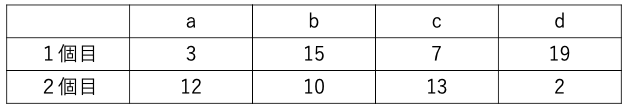
\includegraphics[width=9cm]{2wariate.png}
  %\caption{多重集合の割り当て表}
%\end{figure}

\begin{figure}[H]
  \centering
  \includegraphics[width=7cm]{tajuhash.png}
  \caption{割り当て値の修正}
\end{figure}

\section{動的に変化する集合に対する類似度計算}
最近では動的に変化する集合に対する類似検索も注目されている.ストリームデータとは時間と共に変化するデータであり,直近のw個の要素をスライディングウインドウとして,動的に変化する集合とみなせる.そして、ストリームデータの類似検索は,集合の要素が変化するため,毎時刻ハッシュ値の再計算が必要となる.


\subsection{Datarらによる手法}
Datarら\cite{Datar}は時間と共に変化する集合に対するハッシュ値更新を効率よく行う方法を提案した.
Datarらの手法は,将来的に最小値になり得ない要素を削除,残りをMinlistで管理し,Minlistの最小値をハッシュ値とするという方法である.最小値の候補集合の作り方は,図3のように,ある要素より新しくスライディングウインドウに入ってきた要素が小さい値を持つ場合,将来その要素の値が最小値になる可能性なく,最小値になる可能性のある要素だけの集合Minlistを作成する.このように作成したMinlistは元の集合より小さくなるため,類似度を高速に計算することができる.
しかし,この手法は多重集合で取り扱うことができない.
\begin{figure}[H]
  \centering
  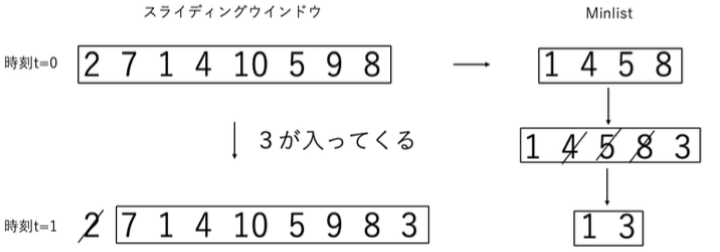
\includegraphics[width=10cm]{Minlist.png}
  \caption{最小値の候補リストMinlistの作成}
\end{figure}

\begin{figure*}[t]
    \begin{tabular}{cc}
      %---- 最初の図 ---------------------------
      \begin{minipage}[t]{0.5\hsize}
        \centering
        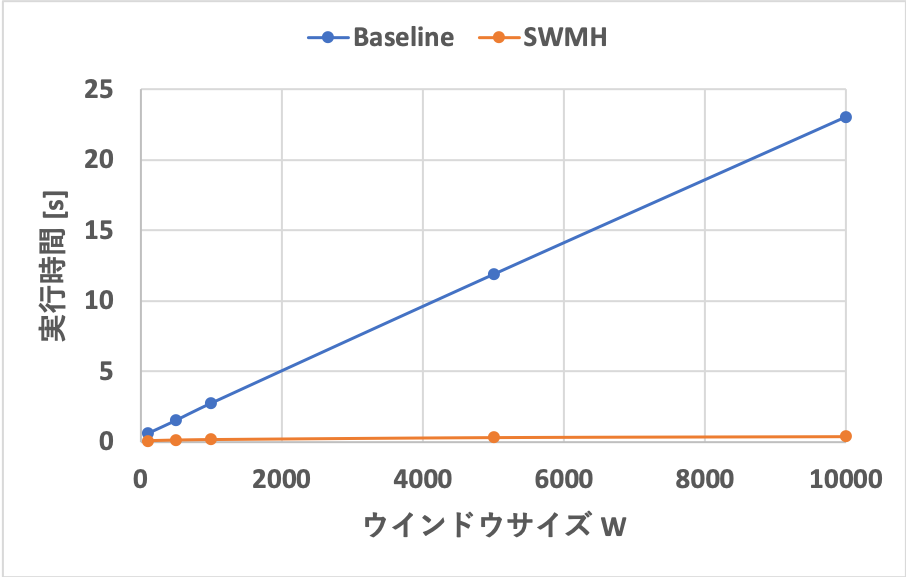
\includegraphics[width=8cm]{SW_jinko.png}
        \caption{人工 dataset}
        \label{fig:jikken1_1}
      \end{minipage}
      %---- 2番目の図 --------------------------
         \begin{minipage}[t]{0.5\hsize}
        \centering
        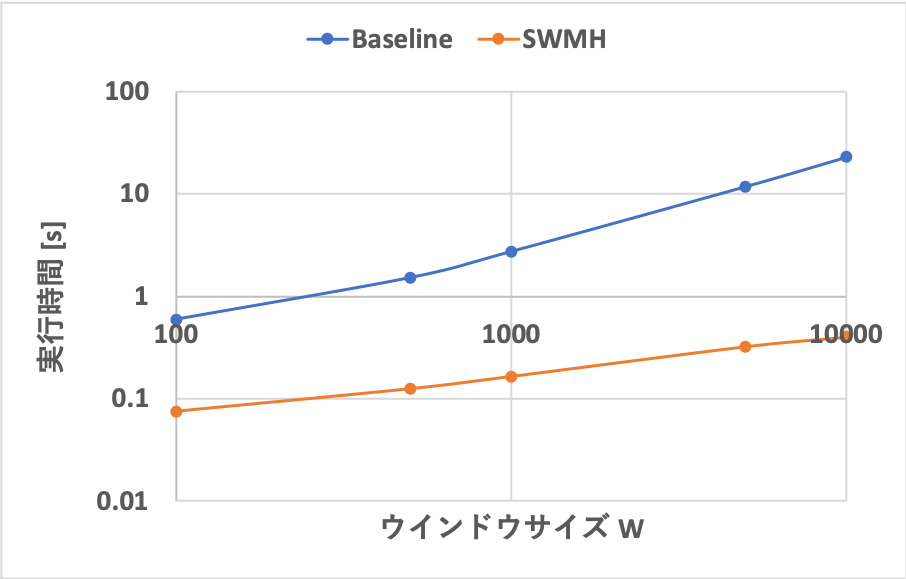
\includegraphics[width=8cm]{jikken1_1_taisu.png}
        \caption{人工datasetにおける対数グラフ}
          \label{fig:jikken1_taisu}
      \end{minipage}
      %---- 図はここまで ----------------------
    \end{tabular}
  \end{figure*}
  
    

  
  
\subsection{多重集合の難しさ}
多重集合では,スライディングウインドウ内の個数によって,ラベルの割り当て値が変化する.そのため、Minlistを作る上で,問題点が二つある.1つ目は,Minlist内に,同一要素が出現し,Minlistが長くなること.2つ目は、割り当て値の変化により,最小値が変わる可能性があり,最小値になり得るかの判断が難しくなることである.


\section{SWMH}
本研究では,Datar[1]らのハッシュ値更新のアルゴリズムを動的多重集合に拡張する手法を考案した.

提案手法の特色は2つである.

(1)同一アルファベットに対する割り当て値を修正し,Minlist内に同一アルファベットが1つしかないことを保証する.ここでは,割り当て値を修正するが,それによって,集合に対するハッシュ値は変化しない.

(2)最小値になり得ない要素を割り当て値の変化があっても特定可能にした.

\subsection{割り当て値の修正}
Minlist内の同一アルファベットの要素を1つにするために,割り当て値の修正を行った.修正方法は.同じアルファベットの中で,$i$番目の割り当て値より$i+1$番目の割り当て値が大きければ修正するという方法である.
\begin{equation}
if (\pi(\alpha_i)<\pi(\alpha_i+1))\{
if \pi(\alpha_i+1)=\pi(\alpha_i)
\}
\end{equation}


\begin{figure}[H]
  \centering
  \includegraphics[width=8cm]{syusei.png}
  \caption{最小値の候補リストMinlistの作成}
\end{figure}

\subsection{最小値となり得ない要素の発見方法}
Minlistにおいて,
到着したアルファベット:$\alpha$,Minlist内の要素:$\beta$,$\beta$よりあとに到着した$\alpha$の個数:$n$,割り当て値:$\pi$として,
$\beta$よりあとに到着した$\alpha$の個数に応じた$\pi$により,将来的に最小値になり得るかどうか判断する.

\begin{equation}
if (\pi(\alpha_n)<\pi(\beta))\{
\beta をMinlistから削除
\}
\end{equation}



\section{実験評価}
本章ではSWMHを人工データと実データを用いて実験的に評価した.人工データセットはzipf分布に従った長さ100,000の文字列であり,実データセットはconnect datasetとmushroom datasetの2種類のデータからそれぞれ長さ100,000の文字列を生成した.

\subsection{ウインドウサイズ$W$を変えた実験}
ウインドウサイズ$ W = 100, 500, 1000, 5000, 10000$ と変えて提案手法の 実行速度を計測した.人工データ, connect, mushroom いずれのデータセットにおいても,SWMH が Baseline より圧倒的に早かった.図\ref{fig:jikken1_1}, \ref{fig:jikken1_taisu}は人工データの結果である.
BaselineではWに比例して増加していくが、SWMHはlogWに比例して実行時間が増加する.

\section{まとめ}
本研究ではデータストリームに対 するハッシュ値の更新アルゴリズムを取り扱った.スライディングウィンドウに対するMin-Hashのハッシュ 値更新アルゴリズムSWMH を提案し,要素の削除と多重集合を取り扱うことができ、実験評価より効果的であることを示せた.

今後の研究課題として,メモリ使用量の削減のために近似ヒストグラムを用いてハッシュ値を計算する手法の実現することが課題としてある.


\begin{thebibliography}{99}
  \bibitem{Datar}
 Mayur Datar and S Muthukrishnan "Estimating Rarity and Similarity over Data Stream Window" AT\&T Research, Florham Park NJ, USA.
 
\bibitem{Minhash}
A Z Broder, M Charikar, A M Frieze, M Mitzenmacher, "Min-Wise Independent Permutations",Journal of Computer and System Sciences Volume 60, Issue 3, June 2000, Pages 630-659.

\end{thebibliography}
\end{document}
